% Text Parse Tree Example
%
% File:         text-parse-tree.tex
% Author:       Bob Walton (walton@acm.org)
% Date:      	Sun Jan 13 23:31:01 EST 2013
  
\documentclass{minimal}
\usepackage[paperheight=3.5in,paperwidth=3.5in,
            height=3.5in,hoffset=0.05in,
	    voffset=0.05in,left=0in,width=3.5in]{geometry}
\usepackage{color}
\usepackage[usenames]{xcolor}
\usepackage{tikz}
\usepackage{scalefnt}
\usetikzlibrary{arrows}
\usetikzlibrary{shapes}
\begin{document}
\raggedright
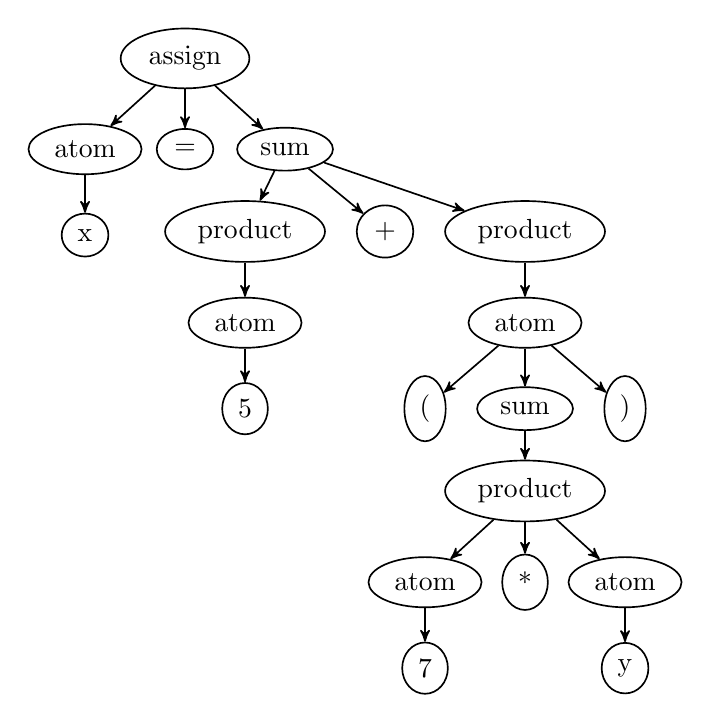
\begin{tikzpicture}[->,>=stealth',auto,
                    node distance=0.5in,semithick]
\tikzstyle{every node}=[draw,ellipse]
\path
node (A) {assign}
(A.south) ++ (-0.5in,-0.3in) node (A1) {atom}
(A1.south) ++ (0in,-0.3in) node (A11) {x}
(A.south) ++ (0in,-0.3in) node (A2) {=}
(A.south) ++ (+0.5in,-0.3in) node (A3) {sum}
(A3.south) ++ (-0.2in,-0.3in) node (A31) {product}
(A31.south) ++ (0in,-0.3in) node (A311) {atom}
(A311.south) ++ (0in,-0.3in) node (A3111) {5}
(A3.south) ++ (0.5in,-0.3in) node (A32) {+}
(A3.south) ++ (+1.2in,-0.3in) node (A33) {product}
(A33.south) ++ (0in,-0.3in) node (A331) {atom}
(A331.south) ++ (-0.5in,-0.3in) node (A3311) {(}
(A331.south) ++ (-0in,-0.3in) node (A3312) {sum}
(A3312.south) ++ (-0in,-0.3in) node (A33121) {product}
(A331.south) ++ (+0.5in,-0.3in) node (A3313) {)}
(A33121.south) ++ (-0.5in,-0.3in) node (A331211) {atom}
(A331211.south) ++ (0in,-0.3in) node (A3312111) {7}
(A33121.south) ++ (0in,-0.3in) node (A331212) {*}
(A33121.south) ++ (+0.5in,-0.3in) node (A331213) {atom}
(A331213.south) ++ (0in,-0.3in) node (A3312131) {y};

\path (A) edge (A1) edge (A2) edge (A3)
      (A1) edge (A11)
      (A3) edge (A31) edge (A32) edge (A33)
      (A31) edge (A311)
      (A311) edge (A3111)
      (A33) edge (A331)
      (A331) edge (A3311) edge (A3312) edge (A3313)
      (A3312) edge (A33121)
      (A33121) edge (A331211) edge (A331212) edge (A331213)
      (A331211) edge (A3312111)
      (A331213) edge (A3312131);
\end{tikzpicture}
\end{document}
